% Preamble of the poster (70 x 100 cm): the palette of the UTDT engineering school (burgundy
% #820A32, ink #2B2B2D) and Montserrat. poster.tex inputs this file, content.tex and layout.tex.
% figures/utdt_logo_*.pdf: the vector UTDT logo, copied from the cover of the UTDT career guide
% 2021 (utdt.edu/Descargas/folletos2021/UTDT_GUIADECARRERAS_2021.pdf). The other figures come
% from poster_figures.py.
\documentclass{article}
\usepackage[paperwidth=700mm, paperheight=1000mm, margin=0mm]{geometry}
\usepackage{fontspec}
\usepackage{unicode-math}
\setmainfont{Montserrat}[
  Extension = .otf,
  UprightFont = *-Regular,
  BoldFont = *-SemiBold,
  ItalicFont = *-Italic,
  BoldItalicFont = *-SemiBoldItalic,
]
\newfontfamily\heavyfont{Montserrat}[Extension = .otf, UprightFont = *-ExtraBold]
\newfontfamily\boldfont{Montserrat}[Extension = .otf, UprightFont = *-Bold]
\setmathfont{FiraMath-Regular.otf}
\usepackage{xcolor}
\usepackage{graphicx}
\usepackage{qrcode}
\usepackage{tikz}
\usetikzlibrary{calc}
\graphicspath{{figures/}}

\definecolor{burgundy}{HTML}{820A32}
\definecolor{ink}{HTML}{2B2B2D}
\definecolor{ink2}{HTML}{5E5E63}
% Colors of the three oracles, as in the plots. The gray of the full tree is too light for text,
% so the captions name the full tree in the caption color.
\definecolor{full}{HTML}{B4B4B8}
\definecolor{interval}{HTML}{008C9A}
\definecolor{method}{HTML}{820A32}

\pagestyle{empty}
\setlength{\parindent}{0pt}
\setlength{\parskip}{0pt}
\hyphenpenalty=10000
\exhyphenpenalty=10000
\color{ink}

\newcommand{\bodytext}{\fontsize{23}{31}\selectfont}
\newcommand{\smalltext}{\fontsize{20}{26}\selectfont}
\newcommand{\tinytext}{\fontsize{17}{22}\selectfont}
\newcommand{\captiontext}{\tinytext\color{ink2}}
\newcommand{\tablefont}{\tinytext}

% TikZ sets \spaceskip in em of the font size of the node: this restores the spacing of each font.
\newcommand{\resetspaces}{\spaceskip=0pt\xspaceskip=0pt\relax}
\tikzset{every node/.append style={execute at begin node=\resetspaces}}

% Absolute placement: \placeblock{x}{y}{width}{content}, in mm from the upper left corner.
\newcommand{\placeblock}[4]{%
  \node[anchor=north west, inner sep=0pt, text width=#3mm]
    at ($(current page.north west) + (#1mm, -#2mm)$) {\resetspaces\raggedright #4};}

\newcommand{\bib}[1]{\par\vspace{0.6mm}\hangindent=9mm\hangafter=1\makebox[9mm][l]{[#1]}}
\newcommand{\tabhead}[1]{{\bfseries #1}}
\newcommand{\collabel}[3]{\makebox[#1][c]{\textcolor{#2}{\bfseries #3}}}

% Big number with its caption: \bignumber{width}{color}{number}{caption}.
\newcommand{\bignumber}[4]{%
  \begin{minipage}[t]{#1}\resetspaces\raggedright
    {\heavyfont\fontsize{84}{88}\selectfont\color{#2}#3\par}
    \vspace{2mm}
    {\smalltext #4\par}
  \end{minipage}}

% The three slanted bars of the UTDT isotype, as the mark of a section heading:
% \stripes{height in mm}{color}.
\newcommand{\stripes}[2]{%
  \tikz[baseline=0pt, x=#1mm/9, y=#1mm/9]{%
    \foreach \i in {0, 1, 2}
      \fill[#2] (\i*4.3, 0) -- ++(2.5, 0) -- ++(4.3, 9) -- ++(-2.5, 0) -- cycle;}}

% The three meshes with their labels on top: \Teaser{width in mm}. The label boxes follow the
% widths of the three panels of figures/teaser.png.
\newcommand{\Teaser}[1]{%
  {\fontsize{26}{32}\selectfont
   \collabel{\dimexpr#1mm*2537/10000\relax}{ink}{\TeaserA}%
   \collabel{\dimexpr#1mm*4601/10000\relax}{ink}{\TeaserB}%
   \collabel{\dimexpr#1mm*2862/10000\relax}{ink}{\TeaserC}\par}
  \vspace{3mm}
  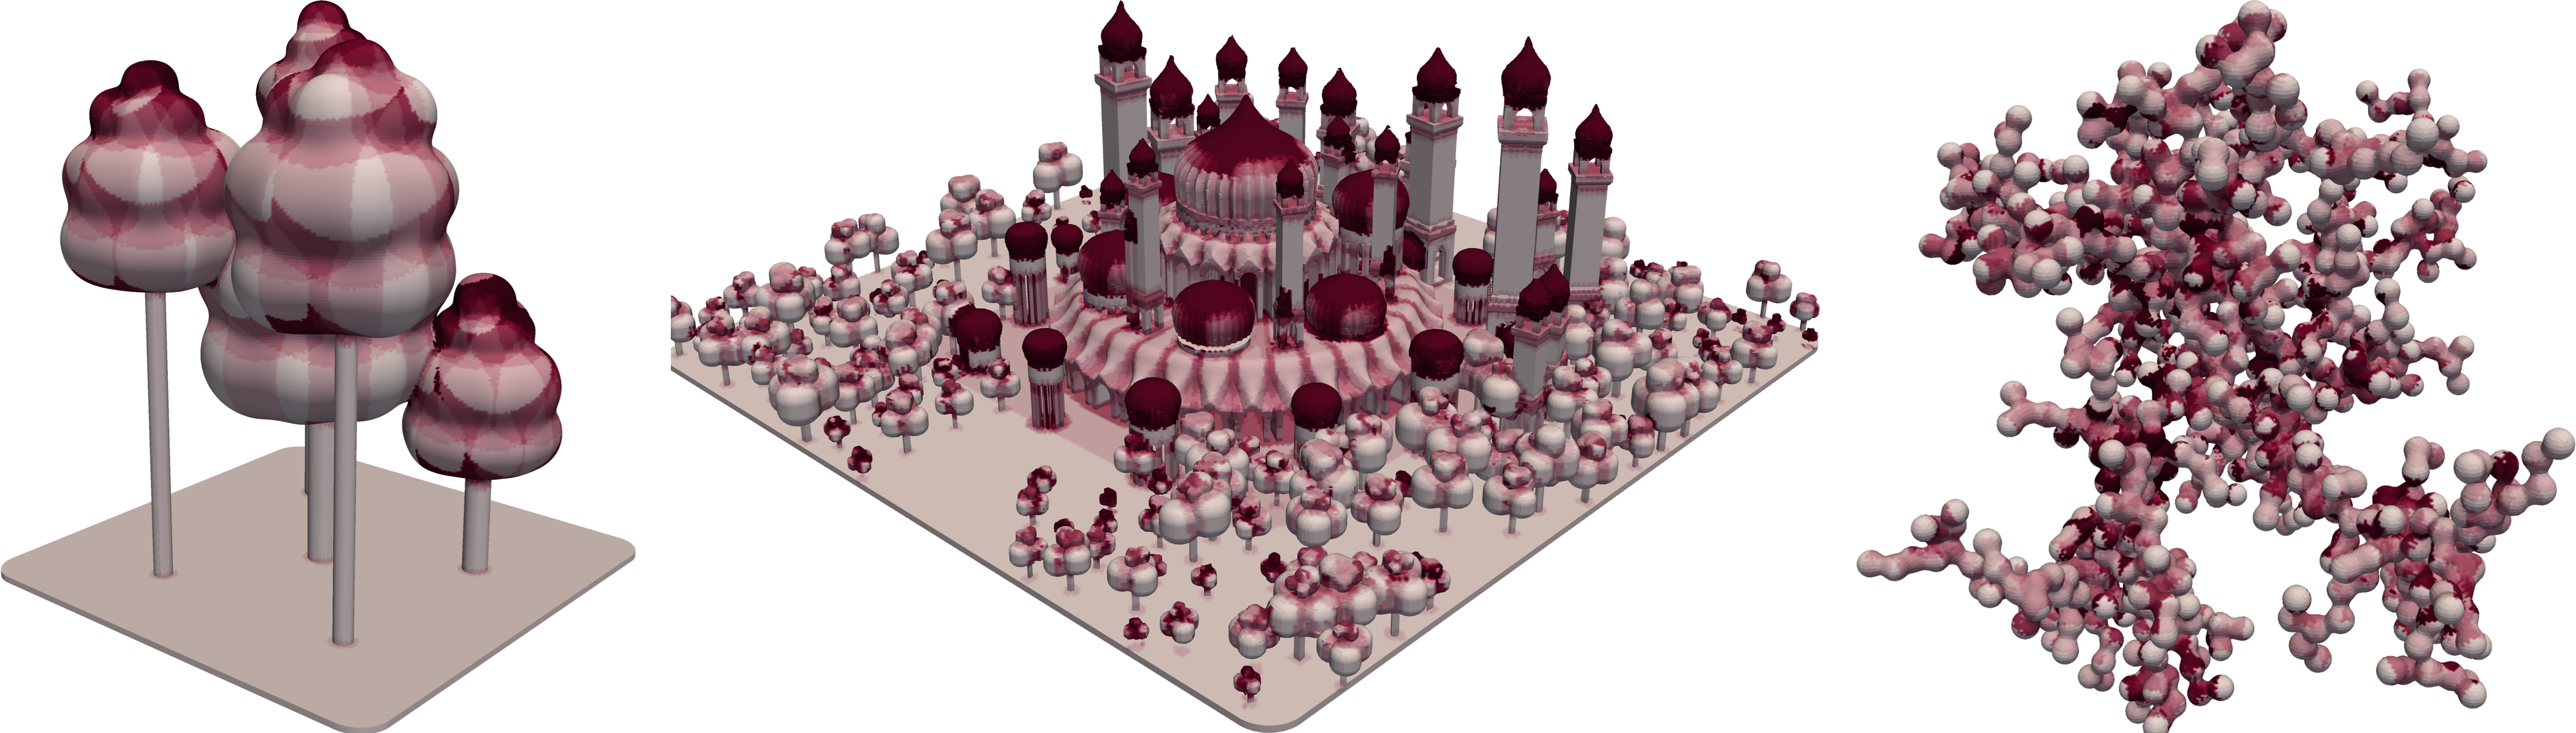
\includegraphics[width=#1mm]{teaser.png}\par}
% Color scale of the meshes: \Scale{width of the bar in mm}.
\newcommand{\Scale}[1]{\ScaleText\hspace{5mm}\raisebox{-3mm}{
\includegraphics[width=#1mm]{colorbar.pdf}}}
\newcommand{\QR}[1]{\qrcode[height=#1]{https://github.com/Lucas-Allara/Lipschitz-pruning-meshing}}
